\documentclass{report}

% cool tables
\usepackage{booktabs}
\newcommand{\ra}[1]{\renewcommand{\arraystretch}{#1}}

\newcommand{\colorA}{\cellcolor{green!100}}
\newcommand{\colorB}{\cellcolor{green!60}}
\newcommand{\colorC}{\cellcolor{yellow!75}}
\newcommand{\colorD}{\cellcolor{orange!90}}
\newcommand{\colorE}{\cellcolor{red!80}}
% images
\usepackage{graphicx}
\usepackage{tabularx}
\usepackage{rotating}
\usepackage[table]{xcolor} 
\usepackage{gantt}
\usepackage{hyperref}
\usepackage{longtable}

\usepackage[T1]{fontenc}
\usepackage{titlesec}

% black square
\usepackage{amsmath}
\usepackage[parfill]{parskip}

%numbers
%\renewcommand\thesection{\arabic{section}}
\pagenumbering{arabic} 

\title{
	\hrule
    \normalsize \textsc{Customer Driven Project}\\
    \Huge Rock Concert Audience as a Screen\\[10pt]
    \normalsize Project Report\\[10pt]
    Netlight AS
    \hrule
    }  
\author{Agnethe Soraa,
Tomas Dohnalek,
Jan Bednarik,
Milos Jovac \\
\normalsize Project adviser: Anh Nguyen Duc}
\date{\today}

\definecolor{gray75}{gray}{0.75}
\newcommand{\hsp}{\hspace{20pt}}
\titleformat{\chapter}[hang]{\Huge\bfseries}{\thechapter\hsp\textcolor{gray75}{|}\hsp}{0pt}{\Huge\bfseries}

\begin{document}
\maketitle
\chapter*{Abstract}
This document gives an insight into the details of planning, preliminary research, requirements, design, actual implementation and evaluation of prototype product named \emph{Digital Lighter}.

The resulting application gives a rock concert audience an opportunity to take part in an active manner during a concert. 
All that is needed is a smart phone.
During the concert the audience is instructed to start the Digital Lighter application, connect to a server, and then raise their hands with the smart phone's screen toward to the stage. This is similar to holding up a lighter. 
Each screen then becomes a pixel on a giant screen, and a video can be played on it.

This is a proof of concept task covering all main problems of the domain.





\chapter*{Preface}
%This report is one of the deliverables in the course TDT4290 Customer Driven Project, which given by Department of Computer and Information Science at the The Norwegian University of Science and Technology, in the fall of 2013. Based on this project, the group's work will be evaluated and graded by the appropriate personnel in charge of the course. 
We would like to thank our teaching supervisor, Anh Nguyen Duc, for regular input and guidance. 
We would also like to give a special thanks our customer, Peder  Kongelf from  Netlight consulting, who has given us the opportunity to work on such an interesting project, and also for being enthusiastic and helpful throughout the whole course.

\tableofcontents
\setcounter{page}{3}

\chapter{Introduction}
%\section{General information}

\section{Structure of report}
\begin{tabular}{l|p{10cm}}
\textbf{Chapter} & \textbf{Description} \\
\hline
Chapter 1 & The introduction chapter introduces the problem, and introduces the members and stakeholders of this project.
This chapter also explains the motivation and goals. \\
\hline
Chapter 2 &  The preliminary Study chapter describes the work and research done. This chapter describes alternative solutions, and an evaluation these solutions. \\
\hline
Chapter 3 &  The planning chapter describes the project plan, the organization, quality assurance and planned workload.  \\
\hline
Chapter 4 &  The requirements chapter describes the requirements, both functional and non-functional. It also describes Use cases for the system. \\
\hline
Chapter 5 &  The test plan chapter contains the approach for testing with the overall test plan for the project.\\
\hline
Chapter 6	 &  The architecture chapter explains the structure of the system, and how it is put together. \\
\hline
Chapter 7	 &   The tools and strategy chapter describes the different tools we chose to use for this project.\\
\hline
Chapter 8-14 	&  In the sprint chapters the reader can see how the product has developed during the time of the project. This includes planning, architecture, the implementation, testing and evaluation of the sprint. \\
\hline
Chapter 15 	 &  The testing chapter describes the different tests. Everything from unit testing to acceptance testing. \\
\hline
Chapter 16 	 &  Evaluation chapter includes the team dynamics, risk evaluation, an evaluation of the customer, supervisor and of course the task. \\
\hline
Chapter 17 	 &  Conclusion chapter sums up the project, and discusses the solution, and looks at further work. \\
\hline
Chapter 18 	 &  The referances chapter contains references. \\
\hline
Chapter 19 	 &  This chapter contains attachments. \\
\hline
Appendix 	 &   The appendix contains user manual, installation guide, meeting minutes and more.\\

\hline
\end{tabular}
\section {Terminology}
\section{Project and project name}

The customer wants a product to make the audience as a screen on a rock concert. We decided to name the product "digital lighter". We agreed on this name because this product digitalizes the concept from "the old days", where the crowd at a concert held up lighters, to create a special atmosphere. 

\section{Project purpose and concept}

The audience members at a rock concert should be able to download a simple application to their cell phone, and register this through a simple GUI.
Behind the artist on stage there is a screen, with a simple camera on top. 
The camera is taking pictures of the audience. 
At special occasions the audience will be instructed, by the artist, to hold up their phones with the screen towards the stage. 
The mobile is a replacement for the lighter.  

On control a signal the application will fill the entire mobile screen with a single color.
The control signal can as an example say: " all pixels white". 
The signal will be specific for each application.
Each mobile will be a pixel in a larger picture, which will be presented on the big screen. 
What kind of picture the audience can create will depend on the number of people in the audience.   

As a motivation for the audience to hold up their phone, the camera on top of the screen will take pictures of the audience.
In that way the audience can see a reflection of them selves, and see what kind of picture they are creating together.

\section{Project goal}
\section{Stakeholders}
\subsection{Customer}
Netlight AS is a consulting company engaged in IT and management. Their field of expertise is within IT management, IT governance, IT-strategy, IT-organization and IT-research. They deliver unique solutions based on their customers requirements. They operates throughout Europe with offices in Stockholm, Oslo, London, Munich and Helsinki. The company was founded at 1999 and employs to 500 employees. 
\subsection{Customer contact}
Peder Kongelf will be our contact person in Netlight. We will have weekly meetings with him to make sure the project is going in the right direction, and of course get opportunities to ask questions. This way we will get a better understanding of the project.

\subsection{Development team}
 The development team's role is, first of all, to meet all requirements presented by the customer and IDI. We are responsible for development of the project. We are also responsible for writing all the documentation for this course.  Our interest in the project is to receive experience with new technologies and project management, as well as to receive satisfactory grading. The project was intended for 5-7 students,but we are only 4 members in our team. This will, in some way, affect what the team can manage towards what was expected when the project was put together.

\subsection{Supervisor}
\section{Project background}

 


\chapter{Planning}
%\section{Project plan}
\section{Methodology choice - Scrum}
\section{Organization}
\section{Risk Management}
\section{Quality Assurance}
\section{Measurement of project effects}
\section{Duration and workload}
\section{Gantt diagram}
You can see the Gantt chart in figure \ref{fig:gantt}.
\begin{figure}
    \begin{center}
        \caption{Gantt Chart: Allocation of sprints into weeks.}
        \label{fig:gantt}
        \begin{sideways}
            \begin{gantt}{9}{14}
                \begin{ganttitle}
                   \titleelement{Week}{14}
                \end{ganttitle}
                \begin{ganttitle}
                   \titleelement{1}{1}
                   \titleelement{2}{1}
                   \titleelement{3}{1}
                   \titleelement{4}{1}
                   \titleelement{5}{1}
                   \titleelement{6}{1}
                   \titleelement{7}{1}
                   \titleelement{8}{1}
                   \titleelement{9}{1}
                   \titleelement{10}{1}
                   \titleelement{11}{1}
                   \titleelement{12}{1}
                   \titleelement{13}{1}
                   \titleelement{14}{1}
                \end{ganttitle}
                \ganttbar{Sprint 0}{0.5}{1.5}
                \ganttbarcon{Sprint 1}{2}{2}
                \ganttbarcon{Sprint 2}{4}{2}
                \ganttbarcon{Sprint 3}{6}{2}
                \ganttbarcon{Sprint 4}{8}{2}
                \ganttbarcon{Sprint 5}{10}{2}
                \ganttbarcon{Sprint 6}{12}{1.5}
            \end{gantt}
        \end{sideways}
    \end{center}
\end{figure}

\subsection{Description ?}
\subsection{Result schedule ?}
\section{Roles}
\section{Version Control}
\section{Textual documentation}


\chapter{Preliminary studies}
%\section{Similar projects}
\section{Market investigation}
\section{Existing technologies and frameworks}
\section{Evaluation of alternative solutions}
\section{Outcome of research - Our decision}
\section{Constraints}
We are developing this project under few technical resource, time and knowledge limitations.
Our biggest limitation is the image processing part.
Half of the team has no experience with this and the other half has little experience.
Their experience is mostly theoretical information about the subject and practical experience is preferred. 

We are aware of this limitation and our plan is to learn by doing.
We are going to start developing and teach ourself while coding.
We chose this approach because we do not want to spend more time than necessary doing research.
Another limitation is lack of experience with Mobile development within the
development team. All of the team members have Android phones, and to be
able to test our application, we have to develop an Android application. Only
one team member have experience with this.

If we are not scaling down the project then we do not have all necessary resources to test the system. As an example we do not have a huge audience.
Also we do not have access to a big screen etc. This is also a limitation.
As this course last for a 13 weeks, it is normal that we have to make some
trade-offs. This project is technically difficult, and there is a limited amount of
time.
\section{Chosen development technologies??}
\section{Evaluation criteria}

\chapter{Requirements}
%\section{Description}
The product can be logically divided into two applications -- server side  and client side.
Each application will be used by different kind users and for better distinguishing of all terms we feel need to define them.

\section{Definitions}
In this section there will be defined and described actors in requirements to avoid misunderstandings. Since our customer namely specified the domain that we should focus on we named the actors as follows.

\paragraph{User} is a participant of concert who wants to actively take part in show and he can download client application.

\paragraph{Concert Manager} or simply \textbf{Manager} is a person who controls what media should be played on screen made from mobile phone's of users. 
He can also manage other general settings.

\paragraph{Client} or \textbf{Client side} is an application controlled by user and provides him opportunity to be part of the screen by displaying figures on his mobile.

\paragraph{Server} or \textbf{Server side} is and application controlled by manager and provides him opportunity to change the media displayed on screen.

\section{Business Requirements}
\subsection{Functional}

\begin{table*}[!h]\centering
\caption{List of all chapters and short description. }
\label{tab:req_func}
\def\arraystretch{1.3}
\begin{tabularx}{\textwidth}{llX}
\toprule[1mm]
\textbf{ID} & Name & Description\\
\midrule
\phantomsection\label{req_F1}\textbf{F1} & Client behavior & Client must be able to receive commands from the server and display color according to the instructions.\\
\textbf{F2} & More servers & An user can specify to which server (concert stage) he wants to connect.\\
\textbf{F3} & Localization & Server must be able to detect mobile device's positions using image processing.\\
\textbf{F4} & Core & Server should be able to display media through a few (a least 3) mobile phones' screens.\\
\textbf{F5} & Media selection & A manager can choose which media should be played on screen made from mobile phones' screens.\\
\textbf{F6} & Attendance & Number of connected devices to server must be displayed in server application. \\

\bottomrule[1mm]

\end{tabularx}
\end{table*}

\subsection{Non-functional}

\begin{table*}[!h]\centering
\caption{List of all chapters and short description. }
\label{tab:req_nonfunc}
\def\arraystretch{1.3}
\begin{tabularx}{\textwidth}{llX}
\toprule[1mm]
\textbf{ID} & Name & Description\\
\midrule
\textbf{N1} & Server-client architecture & Application must work as a server and client architecture.\\
\textbf{N2} & Platform & Audience application must work on at least one mobile platform.\\
\textbf{N3} & Deployment & Application must be deployed to relevant mobile application store.\\
\textbf{N4} & Scalability & The application must be scalable - it must work with different count of mobile phones.\\
\textbf{N5} & Generality & The application must be prepared for future using outside of rock concert domain.\\
\textbf{N6} & Delivery & Final product must be finished until 21st of November 2013 and presented to the committee and the customer.\\
\bottomrule[1mm]

\end{tabularx}
\end{table*}
\section{Use case diagram}
In the figure bellow is shown use case diagram \ref{img:usecase} of the whole system.

\begin{figure}[h]
    \begin{center}
    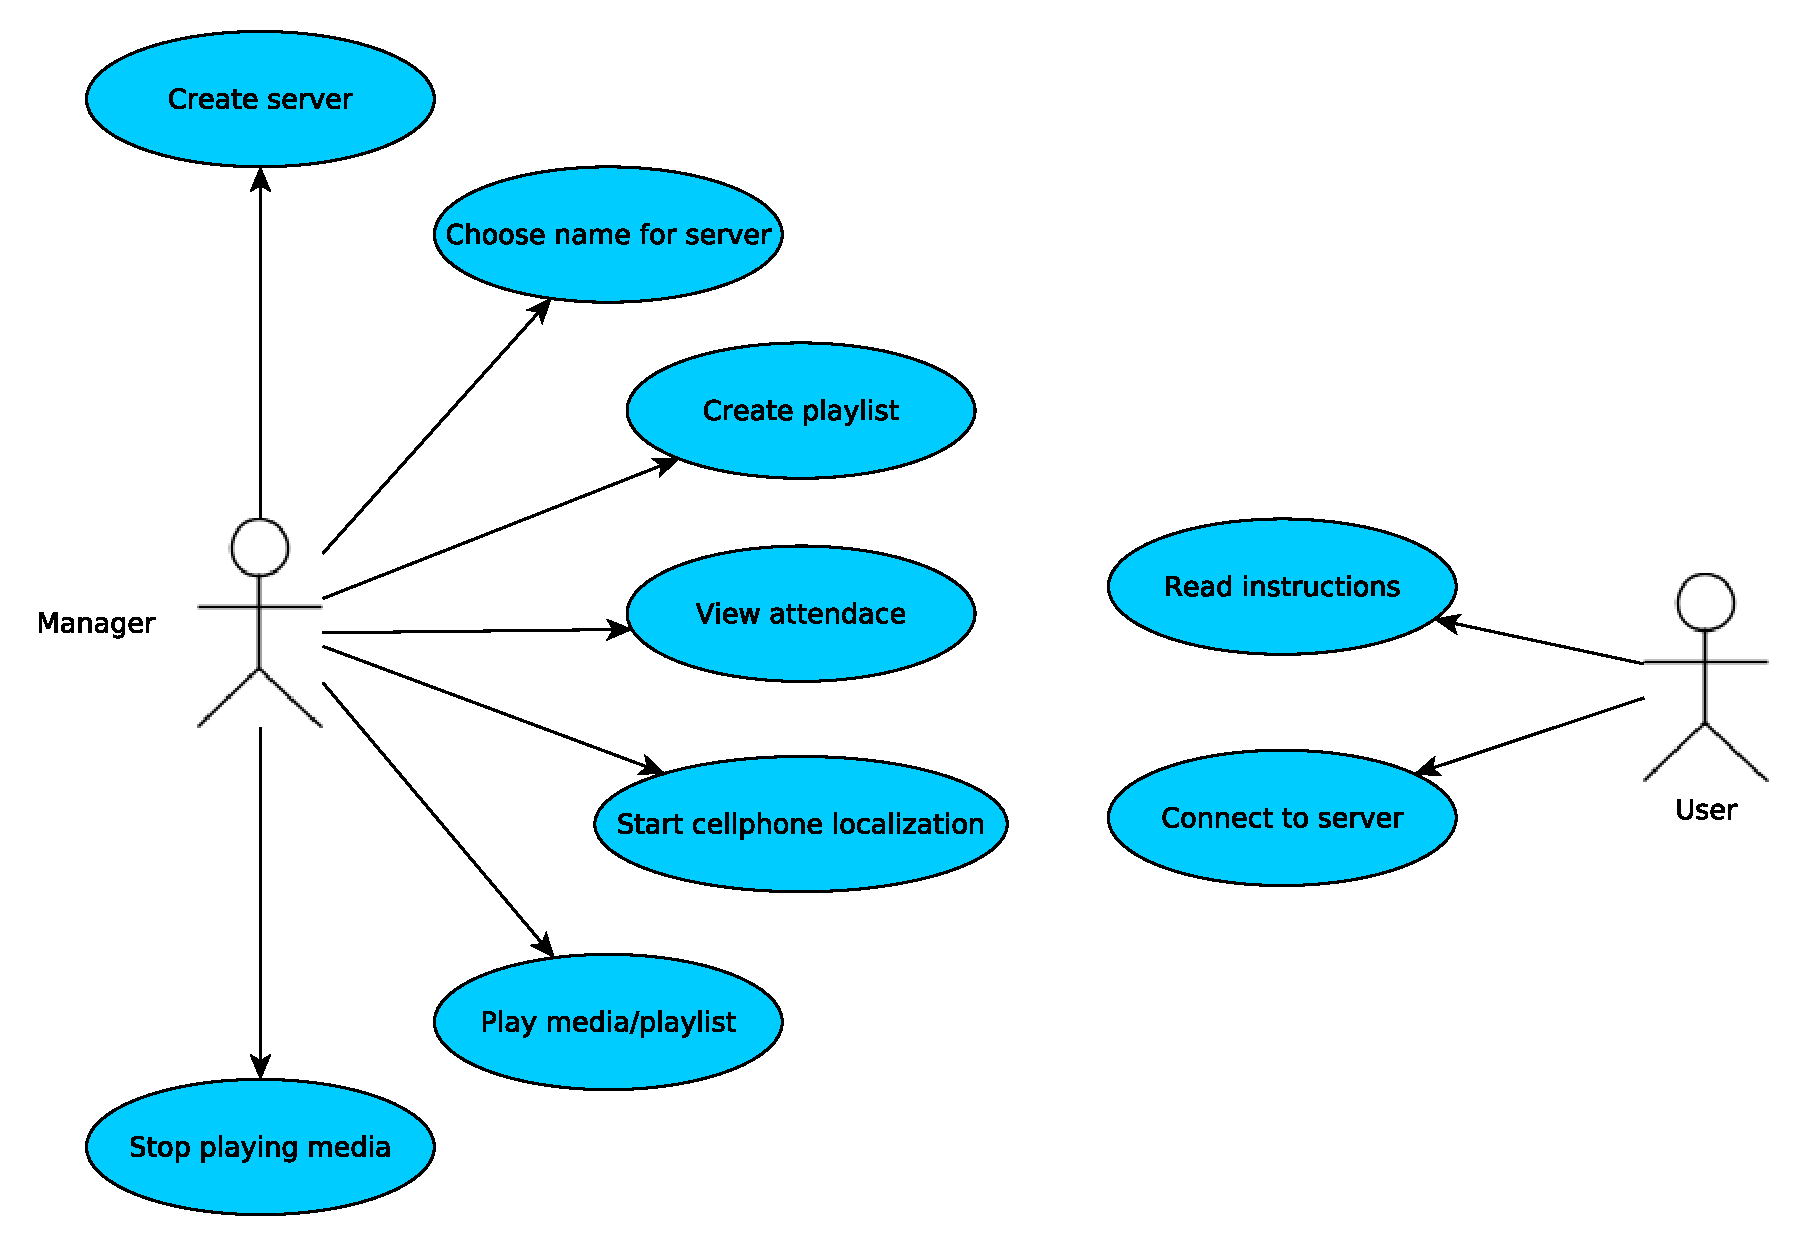
\includegraphics[scale=0.4]{images/usecase.pdf}
    \caption{Use case diagram for both actors User and Manager.}
    \label{img:usecase}
    \end{center}
\end{figure}

%\begin{table*}[!h]
%	\def\arraystretch{1.25}
%	\caption{User stories selected for Sprint 0. }
%	\label{tab:usecase1}
%	
%	\begin{tabular}{p{\textwidth}}
%		\toprule[1mm]
%		\textbf{Use Case detail: Create playlist} \\
%		\midrule	
%		Actors: Manager \\
%		Conditions:
%		
%		\begin{enumerate}
%			\item Manager had created server.
%		\end{enumerate}
%		\bottomrule[1mm]
%	\end{tabular}
%\end{table*}

\section{Summary}


\chapter{Testplan}
%This chapter will introduce the overall test plan for this project. 
The purpose of this chapter is to structure the way tests are performed and recorded. There should also be assigned responsibilities for the testing processes. 
The test plan describes the scope of the overall test effort and provides a record of the test planning process. 
This is the strategy that will be used to verify and ensure that a product or system meets its design specifications and other requirements. 

\section{Approach}
\section{Templates}
\section{Responsibilities}

\section{Test criteria} 
%A test is considered passed when it achieves the expected result. A test will be considered to have failed if the result of the test differs from the expected one.


\chapter{Software Architecture}
%In this chapter, product architecture is described using 4 + 1 architectural view model. It is based on the multiple concurrent views and therefore better explanation of architecture can be provided.
Only high level design will be presented in this chapter and in each sprint, specific, detailed architecture will be described.
The design is made with emphasis on generality, therefore it is possible, that in particular sprints in the architecture section it will be adapted to specific situation.

Since some design patterns were used, the purpose of using specific pattern and its advantages will be discussed in the end of this chapter.

\section{4 + 1 view model}
\subsection{Logical view}
The description of the functional requirements of the architecture. The client and the server are decomposed into a set of key abstractions, taken(mostly) from the problem domain, in the form of objects or object classes.

\subsection{Development view}
\subsection{Process view}
The process view shows concurrency and distribution of a system and system's processes.
It can also show communication between these units.
Process view can be described by activity diagrams.

You can activity diagrams in Figures \ref{fig:activity_diagram_server} and \ref{fig:activity_diagram_client}. Note, that client application is sending signal action \emph{connect to server}, which is connected to server's event action \emph{new client connected}. 
 All clients connections are stored in datastore \emph{client list} and particular actions require all client connections to be able to send any information to clients.

\begin{figure}[H]
	\centering
		\includegraphics[width=16.2cm]{softwareArchitecture/activity_server.pdf}
	\caption{Activity diagram of server application}
	\label{fig:activity_diagram_server}
\end{figure}

\begin{figure}[H]
	\centering
		\includegraphics[width=16.2cm]{softwareArchitecture/activity_client.pdf}
	\caption{Activity diagram of client application}
	\label{fig:activity_diagram_client}
\end{figure}


\subsection{Physical view}
The physical view \cite{Kruchten:1995:VMA:624610.625529} describes a mapping of software onto hardware. 
It takes into account non-functional requirements of the system and it can be described by deployment diagrams.

Deployment diagram depicting physical view can be seen in Figure \ref{fig:architecture_deployment_diagram}.
According to requirement \refreq{N1}, there are two executable files deployed; one deployed to client device and second to server device.
There is also need for NTP\footnote{http://ntp.org/} server, which will maintain all connected devices synchronized.
To generalize the architecture design, the \emph{camera} device is treated as a separate device, which will only send its output to server device.

\begin{figure}[H]
	\centering
		\includegraphics[width=15cm]{softwareArchitecture/deployment-diagram.pdf}
	\caption{Deployment diagram}
	\label{fig:architecture_deployment_diagram}
\end{figure}

\subsection{Scenarios}
Use case diagrams can be considered as scenarios, therefore introduced diagram \ref{img:usecase} in Requirements chapter can be considered as a scenario.

\section{Used design patterns}
\subsection{Strategy}
\subsection{Model-View-Controller}
\subsection{Observer}

\chapter{Tools and strategy}
%\input{toolsAndStrategy/toolsAndStrategy.tex}

\chapter{Sprint 0}
\section{Sprint planning}
We have embraced Sprint 0 as a preliminary sprint, when we can set up all necessary collaboration tools, equipment, prepare templates for meetings and mainly to acquaint ourselves with Scrum methodology. The original plan was to finish sprint 0 on 8th of September, but we have decided to terminate it prematurely due to finishing sprint goals in shorter time than we had expected. Other reason for terminating the sprint was desire to start actually working on the product itself.

The actual user stories are listed in table \ref{tab:sprint0stories}. Since we started to use the software collaboration tool only during the sprint we did not manage to estimate the time needed to complete each story beforehand and thus the column \textbf{Est.} is left empty.

\subsection{Sprint 0 User-stories}

%\begin{longtable}{cX|cc}
%\textbf{ID} & \textbf{Description} & \textbf{Hours estim.} & \textbf{Hours spent} \\
%259 & \LaTeX template for minutes project plan & 5 & 4 \\
%259 & \LaTeX template for minutes project plan & 5 & 4 \\
%\end{longtable}

\begin{table*}[!h]
\caption{User stories selected for Sprint 0. }
\label{tab:sprint0stories}
\def\arraystretch{1.25}
\begin{tabularx}{\textwidth}{cXcc} 

\toprule[1mm]
\multirow{2}{*}{\textbf{ID}} & \multirow{2}{*}{\textbf{Description}} & \multicolumn{2}{c}{\textbf{Hours}} \\
 					& & \textbf{Est.} & \textbf{Sp.} \\
%\textbf{ID} 	& \textbf{Description} 									& \textbf{Est.} & \textbf{Sp.} \\
\midrule
\textbf{259} 	& {\bf I as a developer need to prepare \LaTeX template for minutes, project plan, weekly status report.} 	& 			& \textbf{5} \\
				& \hspace{2em} Meeting minutes	&  & 2 \\
				& \hspace{2em} Project report 	&  & 2 \\

\textbf{245} 	& \textbf{We as a team need to give a project and team name.} 						& 			& \textbf{2} \\
				& \hspace{2em} Team name &  & 1 \\
				& \hspace{2em} Product name &  & 1 \\

\textbf{248} 	& \textbf{I as a developer need to agree on customer, advisor and internal meetings.} 						& 			& \textbf{2} \\

\textbf{247} 	& \textbf{I as a developer need to agree on daily working hours.} 						&  			& \textbf{1} \\

\textbf{243} 	& \textbf{I as a developer need to set up the video conferencing.} 						& 			& \textbf{2} \\

\textbf{249} 	& \textbf{I as a developer need to add goals for Sprint 0.} 						& 			& \textbf{4} \\

\textbf{250} 	& \textbf{I as a developer need to decide which collaboration technologies to use.} 						& 			& \textbf{20} \\

\textbf{258} 	& \textbf{We as a team need to assign roles to team members.} 						& 			& \textbf{1} \\

\textbf{258} 	& \textbf{I as a developer need to write a project plan.} 						&  			& \textbf{90} \\

\textbf{258} 	& \textbf{I as a developer need to research the older reports.} 						&  			& \textbf{30} \\

\textbf{258} 	& \textbf{I as a developer need to summarise the requirements.} 						&  			& \textbf{4} \\
\midrule
				& \textbf{SUM:}		&			& \textbf{161}
 \\																			
\bottomrule[1mm]

\end{tabularx}
\end{table*}

\section{System Burndown}
Since we managed to establish the proper collaboration tool Target Process 3 only during the sprint the software was not able to generate relevant burndown chart. We at least tried to estimate how much time we spent working on each of the user stories listed in table

%\begin{figure}[H]
%	\centering
%		\includegraphics[width=10cm]{sprint0/burn_down_sprint0.png}
%	\caption{Sprint0 Burn Down Chart}
%	\label{fig:sprint0_burn_down_chart}
%\end{figure}


\section{Architecture}
\section{Implementation}
\section{Testing}
\section{Occurring risks}
\section{Retrospective}
\subsection{Pros}
\subsection{Cons}
\section{Evaluation}

\chapter{Sprint 1}
\section{Sprint planning}
After assembling all the tools in Sprint0, we decided to start with the implementation.
As our understanding of task improved, we were able to come up with user stories from the perspective of user, customer, developer and student.
All user-stories were given to the customer so they can be prioritized. 
All but user-stories concerning our student obligations, like writing project plan, minutes, meetings with supervisor and attending lectures.
Those were mandatory and already added as user-stories of sprint1.
On Monday 02.09.2013. we had the meeting with a customer where we estimated time we need for every user story.
The result of that meeting was the list of the rest of the user-stories for sprin1.
All user stories for finishing our first prototype were on the sprint1 list so we also agreed date for presentation and showing the running demo - Thursday 12.09.2013. 
After that ,at a group meeting, we decoupled user-stories into tasks and we were ready to start with the imlementation.

\subsecion {Sprint1 User-stories}

\section{System Burndown}

\begin{figure}[!t]
	\centering
		\includegraphics[width=16cm]{burn_down_chart.jpg}
	\caption{Sprint1 Burn Down Chart}
	\label{fig:sprint1_burn_down_chart}
\end{figure}

\section{Architecture}
\section{Implementation}
\section{Testing}
\section{Occurring risks}
\section{Retrospective}
\subsection{Pros}
\subsection{Cons}
\section{Evaluation}

\chapter{Sprint 2}
%In this chapter the planning and work-flow regarding Sprint 2 will be described. 
Everything from setting our goals to implementation, and testing. At the end we will evaluate whole sprint, and try to answer on following questions: What went well? What could be improved? What should we start doing? 

\section{Sprint planning}
The customer was very satisfied with the video for sprint 1, and suggested recording our future prototypes as well. 
After the successful sprint 1 review we started planning next sprint, sprint 2. Since the customer was very happy with our sprint 1 delivery, he gave us an oppourtunity to decide for ourselves what we wanted to work on this next sprint, and then ask for his approval. 
We decided to focus on multiple client support, and since sprint 1 just focused on connecting one client to the server, then we would also get the opportunity to refine the code we had implemented so far. The customer thought this was a really good idea, because working on this now could help us in future. Catching problems in early phases is much better then discovering them too close to the deadline. Then we might not get the needed time to fix it. Therefore Sprint 2 will focus on adding support for multiple clients connection and sending different signals to different clients. We should revise and improve our code so that we can move on to another core part, image processing, during the next sprint.


In the supervisor meeting the day after the sprint review, we showed our supervisor the project plan. 
We made a document that we called the project plan, but the supervisor wanted these sections to be integrated in the project report instead. Therefore we decided to put some report user stories for this sprint, so that we could integrate the project plan in the report. We also wanted to add the additional sections we needed, for example the sections from Sprint 1. 
Doing a report reasearch and getting a good content is imporant for this sprint, and getting up to speed with the sections. 

\subsection{Duration}
This Sprint will be 2 weeks long. From 16.09.2013 to 29.09.2013.
We agreed on the date for presentation and showing the running demo - Thursday 26.09.2013.
Estimated velocity is 240h since we agreed on 30 working hours per person per week.

\subsection{User-stories}
\LTXtable{\textwidth}{sprint2/stories.tex}

\section{Sprint Goals}
Our goal for Sprint 2 is to deliver a working demo with a more refined core client-server module. 
This still includes registering services, listening for the client and sending simple signals to the client from the server application, but with a more refined code. Of course the client should still scan for the services, connect, receive signals, and play the commands. 
The goal is so sill use the established simple communication protocol. All of the above is extended so it works for several clients connected to the server.

Goals about the report.

\section{System Burndown}
\section{Architecture}
\section{Implementation}
\section{Testing}
\section{Occurring risks}

The risk table 3.3, taken from the risk management section the planning chapter, showes many different risk. 
For this sprint most of the risks did not occur. 
This is mostly because the hardest techical parts, image processing, is planned for the next sprints. 
The user stories this sprint was also very clear, and the customer did not change any of the stories. The time estimation was also very good. 

One of the risks was that team members could get sick. This did not occur, but what did was that that some team members had to be absent in some of the working hours. 
The team solved this by having these team members work more independently, and with more flexible hours.  

\section{Retrospective and Evaluation}
In this section the team will take a look back at sprint 2, and review the sprint. The focus will be on what went well, and goal we achieved. Another focus will also be what we could have done differently, and of course and learn from the this we could have done differently.

\subsection{Pros}
The team reached the sprint 2 goals. The team delivered the demo with our more refined code, and as planned this code supported multiple clients. The clients were able to play the commands the server sent.

The work done in the report is extreamly good. The report is better strucktured now, and the team managed to finish the stories we planned for. We also spent a couple of extra hours to go through the whole report. This was to see if we needed to add more in the spesific sctions, or if we should remove something.  

Even though some member were had other respinsibilities, and had to absent in some of the working hours, the team still got everything done in time for the sprint review. Everyone worked really well independently, as well as in team. 

The sprint planning in this sprint went really well. We had a perfect amount of work, and the hours estimated for ach task, was very realistic, so that was good. 


\subsection{Cons}
The time tracking of each task could have been done better. 
Even though we track our time, the targetProcess3 program dose not have a feature for manually edit the time fracking. 
This means if we forget to do it right away, then the burn down chart wont be as reliable. Since this shows our time tracking we should try to be better at that.

When there is work that needs to be done in the report, the person who writes this section should read terminology, or what other team members have written earlier. This will help to get a better flow for the reader.
This will also save us a couple of hours when we have to refine the report later. 

\chapter{Sprint 3}
%In this chapter planning and work-flow regarding Sprint 3 will be described. 
All from setting our goals to implementation and testing. On the end we will evaluate whole sprint and try to answer on following questions: What went well? What could be improved? What should we start doing?  
% TODO rewrite

\section{Sprint planning}
% TODO

This time we offered customer to have a "pre-demo" video on Thursday 4.10.2013 in our regular meeting.
\subsection{Duration}
This Sprint will be 2 weeks long. From 30.09.2013 to 13.10.2013.
We agreed on the date of presentation and showing the running demo - Thursday 11.10.2013.
Estimated velocity is 240h since we agreed on 30 working hours per person per week.

\subsection{User-stories}
%\LTXtable{\textwidth}{sprint3/stories.tex}
\subsection{Sprint goal}
The goal of this sprint is having a working application on a mobile phone that can work in two modes. 
Input type and output are for both modes common - input is an image or video and output is location of detected mobile phones in a given matrix (e.g. 4x4 matrix) with color that mobile's screen is lighting.
In the first mode, real video from mobile's camera will be treated as an input and on the other hand in the second mode mock data (image/video) are treated as an input.

You can see example of input with matrix 2x2 in image. Appropriate output of image processing and mapping module will be: \texttt{\{blue,[0,0]\}, \{red,[0,1]\}, \{green,[1,1]\}}.

\begin{figure}[H]
	\centering
		\includegraphics[width=7cm]{sprint3/sprint3_goal.jpg}
	\caption{Example of ideal data input for image processing module with 2x2 matrix.}
	\label{img:sprint3_goal}
\end{figure}

\section{System Burndown}
\section{Architecture}
\section{Implementation}
\section{Testing}
\section{Occurring risks}
\section{Retrospective}
\subsection{Pros}
\subsection{Cons}
\section{Evaluation}

\chapter{Sprint 4}
%\label{chap:sprint4}
In this chapter the planning and work-flow regarding Sprint 4 will be described. 
Everything from setting our goals to implementation and testing. At the end the team will evaluate the whole sprint and try on answer the following questions: What went well? What could be improved? 
\section{Sprint planning}

The team with the customer planned how to take the project further on a regular planning meeting.
At this point it was possible to send control signals to multiple clients, and then detect the screens that lit up. 
It was decided that the plan for this sprint was to combine those two modules, and try to display a short animation.
This meant that detection of possible clients' locations must be performed and than connecting its position in a grid with an appropriate socket linked with client.

After this locating, commands to all clients must be continuously send with information, what colors should they lit.
To be more efficient and do not use too much traffic, which could result into delays on network, it was proposed by customer that video should be preprocessed and large chunks of data with timing should be send to clients.

Next, the team with the customer discussed long term planning of the product.
Since this product cannot be finished and deploy for everyday and commercial use due to time restriction, the features included and not included in final prototype were discussed.
The customer proposed two different goals.
One involved mobile device tracking (on rock concert after detection phase, it is probable, that audience wont be static but they will be moving, and therefore if animation should be displayed in proper way, these movements should be detected).
After a short discussion, it was decided that this is a long term goal, which is out of scope of this project.
The focus was put on finishing all core modules and therefore a different goal was adopted.
This goal will be described in Section \ref{sec:sprint4goal}.

As the team wanted the customer feedback more often, it was again settled, than a next pre-delivery demonstration will be made for meeting on 17th of October. 

All implementation related stories for sprint 4 are presented in Table \ref{tab:sprint4stories}.
\begin{table*}%\caption{User stories selected for Sprint 3.}
 \def\arraystretch{1.25}
 \caption{Implementation user stories selected for sprint 3}
   \label{tab:sprint3stories}
 
\begin{tabularx}{\textwidth}{ccXcc}

\toprule[0.5mm]
\multirow{2}{*}{\textbf{ID}} &
\multirow{2}{*}{\textbf{Ref.}} & \multirow{2}{*}{\textbf{Description}} & \multicolumn{2}{c}{\textbf{Hours}} \\
 					& & & \textbf{Est.} & \textbf{Sp.} \\
%\textbf{ID} 	& \textbf{Description} 		& \textbf{Est.} & \textbf{Sp.} \\
\midrule
\textbf{I3.1} 	& \refreq{M4}	& {\bf As a server I need to be able to process images from the real world.}		& 32		& \textbf{28} \\

\textbf{I3.2} 	& \refwbs{wbs_testing}{WBS 6.2}	& {\bf As a server I need to be able to process images from the virtual world.}		& 20		& \textbf{23} \\

\textbf{I3.3} 	&\refreq{M4} 	& {\bf As a server I need to be able to detect one client from its light.} 		& 40		& \textbf{46} \\


\textbf{I3.4} 	& \refreq{M4}	& {\bf As a server I need to detect multiple clients from light.}		 &  5	& \textbf{8} \\


\textbf{I3.5} 	& \refreq{M4}	& {\bf As a server I need to map all available devices to grid.} 			 & 10 & \textbf{10} \\	

\midrule
		
				&& \textbf{$\sum$}		&		107	& \textbf{115}
 \\																			
\bottomrule[0.5mm]
\end{tabularx}
\end{table*}


In sprint 4 the team also planned to work more on the report. 
The plan was to finish sprint 3, since that sprint itself finished the week before. 
It was also wanted to start working on sprint 4 in report.
Since more modules were implemented and their integration must be done, discussion about architecture started to be intensive.
The main goal was to keep architecture as general as possible and open for all future (out of scope) features.
Therefore the idea of architecture become more clear and work on writing architecture chapter could start.
The team where also getting a better understanding of what the end product would look like, therefore it was planned to start working a little bit on the evaluation as well. 
The supervisor also came up with some suggestions for small improvements on the report, which the team planned to follow up.
Also it was decided to make to the user stories more consistent. 
Last but not least, it was also planned to separate the implementation stories from the documentation, and the project management stories.

All the documentation related stories for sprint 4 are presented in Table \ref{tab:sprint4Documentationstories}.
%\caption{User stories selected for Sprint 1.}
\label{tab:sprint1Documentationstories}
\def\arraystretch{1.25}
 
\begin{longtable}{ccXcc}

\toprule[0.5mm]
\multirow{2}{*}{\textbf{ID}} &
\multirow{2}{*}{\textbf{Ref.}} & \multirow{2}{*}{\textbf{Description}} & \multicolumn{2}{c}{\textbf{Hours}} \\
 					& & & \textbf{Est.} & \textbf{Sp.} \\
%\textbf{ID} 	& \textbf{Description} 									& \textbf{Est.} & \textbf{Sp.} \\
\midrule
% === DOCUMENTATION ==========================
\textbf{343} 	&& {\bf As a student I have to work on Project Plan.} 	& 		12	& \textbf{12} \\
							
				
\hline
				&& \textbf{SUM:}		&		?	& \textbf{?}
 \\																			
\bottomrule[0.5mm]
\end{longtable}


All the project management related stories for sprint 4 are presented in Table \ref{tab:sprint4storiesProcess}.
\begin{table*}[!ht]%\caption{User stories selected for Sprint 6.}
\def\arraystretch{1.25}
 
 \caption{Documentation stories selected for sprint 6}
 \label{tab:sprint6storiesProcess}

\begin{tabularx}{\textwidth}{ccXcc} 

\toprule[0.5mm]
\multirow{2}{*}{\textbf{ID}} &
\multirow{2}{*}{\textbf{Ref.}} & \multirow{2}{*}{\textbf{Description}} & \multicolumn{2}{c}{\textbf{Hours}} \\
 					& & & \textbf{Est.} & \textbf{Sp.} \\

%\textbf{ID} 	& \textbf{Description} & \textbf{Est.} & \textbf{Sp.} \\
\midrule


	
\textbf{P6.1} 	&
	\refwbs{wbs_project_management}{WBS 7.1.1}& {\bf As a student I have attend the meeting with the customer} 			& 	?	& \textbf{?} \\
	
\textbf{P6.2} 	&
	\refwbs{wbs_project_management}{WBS 7.1.2}& {\bf As a student I have to attend the meeting with the supervisor} 		& 	?	& \textbf{?} \\

\textbf{P6.3} 	&& {\bf  As a student I have to prepare for the final presenation} 		& 	?	& \textbf{?} \\

\textbf{P6.4} 	&& {\bf  As a student I have to deploy the application on app store} 	& 	?	& \textbf{?} \\
\textbf{P6.5} 	&& {\bf  As a student I have to prepare for submission of the report} 	& 	?	& \textbf{?} \\
\textbf{P6.6} 	&& {\bf  As a student I have to create final demo-video} 	& 	?	& \textbf{?} \\
							
\hline
				&& \textbf{$\sum$}		&		?	& \textbf{?}
 \\																			
\bottomrule[0.5mm]
\end{tabularx}
\end{table*}


% hous all in total: Estimated: 130 + 65 + 42 = 237  Spent: 136+ 36+35= 207

\subsection{Duration}
This sprint is 2 weeks long. From 14th of October 2013 to 27th of October 2013. 
We agreed on the date of presentation and showing the running demo -- on Thursday 25th of October 2013.
Estimated velocity is 200 hours since we agreed on 25 working hours per person per week.

\section{Sprint goal}
\label{sec:sprint4goal}
The goal of this sprint is to have application which integrates already implemented modules.
This application should be able to display using clients a short animation of a traffic light as can be seen in Figure \ref{fig:trafficlight}.
This is in fact prototype 4 -- \emph{Traffic light control} as can be seen in Section \ref{sec:milestones}.

\begin{figure}[h]
	\centering
		\includegraphics[width=10cm]{sprint4/trafficlight.png}
	\caption{Traffic light}
	\label{fig:trafficlight}
\end{figure}

\section{Architecture}
In this section it will be described architecture for sprint 4 using 4+1 view model.
The implementation work can be divided into two logical parts: linking clients' sockets with their position in grid and processing media (animation) into chain of commands for clients.
Therefore the architecture description will be in each view divided into two parts.

\subsection{Logical view}
In Figure \ref{fig:class_diagram_device_sprint4} can be seen class diagram of device locating component.
On the top of the hierarchy there is an interface \texttt{DeviceLocatingStrategy}, which defines common behavior for two classes: \texttt{DeviceMapper} and \texttt{DeviceTracker}.
The first mentioned is an abstract class and defines shared behavior for all (future) types of implementations of linking sockets with positions.
One of these classes is \texttt{DeviceMapperSimple} which uses simple dummy algorithm.
This algorithm simply let lit clients with white color one by one and detects this color.
Detected tile is position of a mobile device.

Class \texttt{DeviceTracker} is class that is used as a getter of list of devices with their positions.
Core of this class is missing, it is only present so it can be extend as a future feature.
Future purpose of this class is to track already detected devices and update their positions during playing media.

\begin{figure}[h]
	\centering
		\includegraphics[width=16.2cm]{sprint4/class_diagram_device.png}
	\caption{Sprint 4 device locating module}
	\label{fig:class_diagram_device_sprint4}
\end{figure}

In Figure \ref{fig:class_diagram_device_sprint4b} you can see class diagram of second component -- media player.
Class \texttt{ImageMapper} is responsible for loading single pictures.
These pictures are used by class \texttt{CommandCreator}, which can create commands generically during run
and as a parameter can be passed number of frames that should be parsed in advance and send to client in single command.
For sending to clients in appropriate moments is responsible instance of class \texttt{MediaPlayer}.
As you can see, the \texttt{MediaPlayer} class keeps an instance of class \texttt{DeviceLocatingStrategy} which servers as a getter for sockets and positions.
\begin{figure}[h]
	\centering
		\includegraphics[width=11.0cm]{sprint4/class_diagram_media_player.png}
	\caption{Sprint 4 media player module}
	\label{fig:class_diagram_device_sprint4b}
\end{figure}


\subsection{Physical view}
In this sprint, no changes were made in physical view.
Therefore you can see the physical view in deployment diagram in Figure \ref{fig:sprint3_deployment_diagram} from sprint 3.

\subsection{Process view} \label{txt:sprint4_processview}
Process view for sprint 4 can be seen in activity diagram in Figure \ref{fig:sprint4_activity_diagram}.
First, to all clients is sent control signal to lit with black color.
After some delay (because of possible network delay, there is need for waiting), all white blobs are detected, this represents \emph{false alarm} blobs.
Next, iterating through all clients starts.
In each iteration to only one clients is sent to lit with white color.
Again, after some delay a new detection is performed and difference between currently detected white blobs and false alarm blobs is calculated.
The difference is a position of client.

It should be mentioned, that both activities \emph{Detect white color} are in fact slightly modified subactivities, which can be seen in Figure \ref{fig:sprint3_activity_diagram}.
Therefore this diagram in Figure \ref{fig:sprint4_activity_diagram} is subactivity of activity \emph{Detect clients location} of Figure \ref{fig:activity_diagram_server}.
\begin{figure}[h]
	\centering
		\includegraphics[width=16.2cm]{sprint4/activity_sprint4.pdf}
	\caption{Sprint 4 activity diagram}
	\label{fig:sprint4_activity_diagram}
\end{figure}

The media player component is from point of process view rather straightforward, and therefore there will be no figure presented.

\section{Testing}
There was no unit testing for device locating component, because mocking of network module, which is needed for this testing was estimated with too high value.
Therefore testing was performed with all modules integrated.
The team focused on finding the lowest value for waiting which can be seen in Figure \ref{fig:sprint4_activity_diagram}.
This value was set on 200 milliseconds due to empirical research.
It should be mentioned, that this value suppose very low delay between sending lit control signal and its performing by client.
Three mobile devices were used for testing purposes.
You can see an example of the form of testing in prototype 4 demonstration video\footnote{\url{http://www.youtube.com/watch?v=6mV5ajoZomI}}.

Media player component did not require connected clients and therefore unit testing could be performed.
For this testing, traffic light media\footnote{\url{https://github.com/dohnto/DigitalLighter/tree/master/source/DigitalLighterServer/assets/3x3/traffic-light}} was chosen.
After verification, component was integrated to the system and integration testing in real situation was performed.

\section{Occurring risks}
In this sprint, working prototype was very close to final product.
Almost all code modules were implemented and integrated and therefore testing of whole prototype could be done quite exhaustively.
Unfortunately there was lack of mobile devices and also the team could not borrowed any router supporting DNS relay.
Both customer and supervisor were asked for advice where to gain required hardware, but only negative or very general hints were provided.
Therefore the testing was performed just with few devices, which cannot be counted as complete.
There is possibility, that server application is going to have problems with large number of clients.

One team member announced very early in the process phase his absence for second week of this sprint.
Since the absence was planned for in advance, the team was able to deal with this problem.
Also the missing member was active beyond working hours.

\section{Customer feedback}
As the team succeeded to implement the most parts of Prototype 4 (see Section \ref{txt:requirements}) the only part left was to create the demonstration of the traffic light, the three (or more) devices ordered vertically displaying red, yellow and green color, the setting reminiscent of the ordinary traffic light. The team managed to finish the implementation in the first half of the sprint so the demonstration video was presented to the customer one week in advance.

The customer expressed his contentment with the goals achieved. He however stated the team should focus more on the speed of detection of the devices. Using current "one-by-one" approach is too time consuming. What is more from now on the team should focus mostly on coming up with the ideas how to present the product in the most immersive way.

On the second meeting during this sprint the team suggested the ideas about what to utilize the created product for. The customer decided to choose the equalizer video effect that would be displayed on the phones while accompanying the played music.

The video presented to the customer can be found on YouTube under the name Prototype 4: \url{http://www.youtube.com/watch?v=6mV5ajoZomI}.

\section{Retrospective}
This section reflects on the past sprint. In order to learn from the mistakes done and thus to improve the workflow it is necessary to answer two essential questions: "What went well" and "What could be improved".
You can see the burn down chart for sprint 4 in Figure \ref{fig:Burn4}.

\begin{figure}[h]
	\centering
		\includegraphics[width=18cm]{sprint4/BurndownSprint4.png}
	\caption{Burn down chart for sprint 4}
	\label{fig:Burn4}
\end{figure}

\subsection{What went well}
All implementation related user stories were finished and as a consequence the goal for sprint 4 and the milestone \emph{Traffic light control} were reached.
The work in implementation part of this project start to escalate and team started to be enthusiastic.

The team was able to prepare and deal with situation, that one member was absent for a whole week.

\subsection{What could be improved}
Stand-up meetings were not that often anymore.
Due to other obligations of all members of team and late attendance during work hours, it was difficult find a common time for these meetings.
Attendance should be more accurate and if absence is known ahead, it should be mentioned to other members.



\chapter{Sprint 5}
%\section{Sprint planning}
\subsection{User-stories}
\subsubsection*{Implementation}
All the functional requirements for sprint 5 are presented in table \ref{tab:sprint5stories}
\LTXtable{\textwidth}{sprint5/stories.tex}

\subsubsection*{Documentation}
All the documentation stories for sprint 5 are presented in table \ref{tab:sprint5Documentationstories}
\LTXtable{\textwidth}{sprint5/storiesDocumentation.tex}

\subsubsection*{Project management}
All the project management for sprint 5 are presented in table \ref{tab:sprint5storiesProcess}
\LTXtable{\textwidth}{sprint5/storiesProcess.tex}
\section{System Burndown}
\section{Architecture}
\begin{figure}[H]
	\centering
		\includegraphics[width=15cm]{images/deployment-diagram-sprint5}
	\caption{Deployment diagram}
	\label{fig:sprint5_deployment_diagram}
\end{figure}
\section{Implementation}
\section{Testing}
\section{Occurring risks}
\section{Customer feedback}
\section{Retrospective}
\subsection{What went right}
\subsection{What to improve}


\chapter{Sprint 6}
%\section{Sprint planning}
\subsection{User-stories}
\section{System Burndown}
\section{Architecture}
\section{Implementation}
\section{Testing}
\section{Occurring risks}
\section{Retrospective}
\subsection{Pros}
\subsection{Cons}
\section{Evaluation}

\chapter{Testing}
%\section{Types}
\section{Unit testing}
\section{Integration}
\section{System testing}
\section{Usability}
\section{Acceptance}







\chapter{Evaluation}
%The evaluation is one of the final phases of this project. In this chapter, we will evaluate different aspects of the projects. 
Here it will be discussed why and how the outcome ended up being what it is today.
This includes how the team worked together, why it gave the result it did, the cooperation with the customer, and how it was working with an overseeing force. Furthermore,we will discuss the issues met during the project, and how the process we used worked for us.
We have chosen to split the evaluation into three major parts, group evaluation, project evaluation and technology evaluation. 
 
 
This is the final phase of this project, the evaluation. Here it will be discussed why and how the outcome
ended up being what it is today.  
The technology evaluation will be a fairly straightforward discussion and evaluation of our experiences with the technology we used in this project.
%_______________________________________________________________________________
\section{Group evaluation}
The group evaluation will discuss the social aspects of the project. 
We will discuss the team dynamics, our goals, how we used our role assignment, risk assessment, the advisor the customer, and other issues regarding group evaluation in general.
The project evaluation will be a discussion of the work process and technical problems we encountered.

\subsection{Team dynamics}

\subsection{Communication}
The communication was done through frequent physical meetings, and if someone had other obligations and they were not able to be precent, then we kept in contact though Facebook. This was a suitable solution for us since the team members were available online nearly all the time. 
This made coordination an easier task, since other members could be consulted at any time. 
Furthermore, our small group size allowed us to get well known with each other, and this made the communication better.

Key words for further writing

working hours and people not showing up in time cuz they did something late at night and then figures it was okay not to show up, then the rest of the group did not show up either.


+pysical meetings
+facebook
+stand ups, could have done more of those
+meetings, did not have weekently, but we asked for them if we neededto

-Not alwas CC in emails to the whole group
-Some members did not get the information when needed 


write something about conflicts resolution?

All in all there wherent personal issues, friends, just discussions regaring solutions to the project. 

\subsection{Goals} 


\subsection{Challanges}

In this section we will elaborate on some of the challenges that we encounter during the project. Some if the issues were minor, and some where lager. The team will in this section reflect on the challanges we had, and why they occured, and what we could have done differently.

\subsubsection{Time}

Throughout the project, time restrictions has been a challange because most of the members in the group have had other projects during the semester. Everyone also had different courses, so suitable working hours for everyone was also a challange. Agnethe had two different projects in addition to the customer driven project. Milos also had another project that was quite time consuming in the beginning. Jan and Tomas also had another project besides the customer driven project, and Jan also wanted to take Norwegian classes. All of this made it hard to find working hours. 

\subsubsection{Language Barriers}


\subsection{Work distribution}

The work distribution was very dynamic. We agreed on what needed to be done, and then group members had to take individual responsibility to perform work on the tasks they were comfortable with.
We could have distributed the work more evenly through out the project. 
It was a little stessful towars the ending of the project. Especially since we had to prioritize making the demo-video in the 5th sprint. Then we had a little trouble with the demo-video, and we had to spend more hours than we first thought. Because of this writing the documentation was a lower priority, and we fell a little behind.  
  
\subsection{motivation}
Motivation turned out to be a major stumbling block in our project. For the
most past, this lack of motivation stems from the complexity of the existing
system we were working on, and the fact that the system was not very well
documented. Throughout the implementation phase, we very often had to ask
our customer for help. This made it ever so slightly demotivating to take on
new tasks, as it meant that our customer told us step by step what you were
12.2. GROUP EVALUATION 137
going to do, where in the system it was going to be done, and how it had to be
implemented. Thus the feeling of independence rarely occurred.
\subsubsection{Effort and estimation}
Throughout the project, time restrictions has been an issue for the group. Most of the 
members in the group have had other group projects during the semester, making it hard to 


\subsection{Role assignment}
As mentioned earlier the role assignment was adapted a bit, so it could fit our project better. Also the roles that was assigned to each group member was more of a guideline, rather than a binding responsibility. This was mainly because or some of the team members this was their first scrum project, and some of the roles requireed more experience and knowlede than the respective goup member had. To solve this problem we often devided the roles over several group members depending on the context and situation. Working with the architechture for example often requireed more than one person responsible. 

When we look back at the role assignment we realize that since we were working with many technologies all of us were unfamiliar in the beginning, it might have been a good idea to make each of the role's responsibility more clear, and maybe spend some time enforcing these responsibilities in the early stages of the project. Also, we should have spent more time finding researching which roles we needed, because some of the roles we assigned we did not use. Even though we decided to embrace this as an equal development team, the roles might have been useful for us. 

These are the roles we assigned, and this is how we evaluated them.

\paragraph{Project Leader}
The project leader was supposed to be responsible for the project progress, and delegate tasks to the other team members. This did not work, because the tasks was prioritized by the customer. If one task was done, the team member had picked the task with the highest priority. All of the team members took responsibility for the progress of the project, and tried to make sure that is went according to the plan. The description also claimed that the Project Leader had final call in arguments, but no group member felt the need to have one person in charge. We chose to embrace this as an equal development team, and that worked well for us.

\paragraph{System Architect}
The system architech was responsible for checiking and analyzing all the layers in the produckt, but this was also something not only one person took responsibility for. 

\paragraph{Scrum Master}
Also the Scrum Master role was assigned to one person originally, but every team member took responsibility for following up on this. It became natural for all of the team members to suggest to have stand ups when we had working hours. It was not always easy too keep track of what the other team members where working on, and this problem occured since the team were not able to have working hours everyday. The reason for this was that the team members had other courses with projects as well, and therefore we were not able to meet up every day. Having the whole team responsible for scrum methodology worked well for us.

\paragraph{Communication Responsible}
This role is the only that was used throughout the whole project was the customer and supervisor contact responsible. Although this was not a high workload, it was easier for both the customer and supervisor to have one person to communicate with when they had questions.  

\paragraph{QA Responsible}
The QA was responsible for the quality of all documents and also the end product, but the whole team felt responsible for delivering a product with good quality. The QA is also supposed to help with determening is stories and acceptance criteria are well defined, and if they satisfy the requirements.The problem we had with this was that it is hard to conduct if the team member responsible is not that experienced with the scrum methodology. A QA is also responsible for organizing testing, and this includes that unit tests are well written, provide developers with high level test cases for the stories, and performing explorotory tesing on early builds, but in our project we did not focus on the testing part. 

\paragraph{Documentation Responsible}
Also this was a role that every team emmber took responsibility for. It was good to have one person resonsible to set up a good structure in the beginning, but when we started writing more of the conents everyone participated where they could. 

\subsection{Risk evaluation}
\subsection{Customer} 
\subsection{Advisor}
%_______________________________________________________________________________
\section{Project Evaluation}
This section will start with an evaluation of the planning phase and our preliminary studies.  
Then we will look at our use of the scrum method, and how we had to modify it for our project, before moving on to a discussion of our conduction of meetings. 
\subsection{Planning}
\subsection{Preliminary Studies}
\subsection{Scrum}
\subsection{Meetings-Summary}
\subsection{Course feedback}
\subsection{Testing}
\subsection{Time usage}
%_______________________________________________________________________________
\section{Technology evaluation}
\subsection{Skype}
\subsection{Github}
\subsection{Facebook}
\subsection{Testflight}
\subsection{Google documents}
\subsection{Latex}
\subsection{TargetProcess3}
\subsection{Technical issues}


\chapter{Conclusion}
%\section{Introduction/Final product/description}
\section{Results}
\subsection{Server-side application}
\begin{figure}[H]
	\centering
		\includegraphics[width=5cm]{conclusion/server_ui.png}
	\caption{Server UI}
	\label{fig:Server_UI }
\end{figure}

\subsection{Client-side application}
\begin{figure}[H]
	\centering
		\includegraphics[width=7cm]{conclusion/user_ui.png}
	\caption{Client UI}
	\label{fig:Client_UI }
\end{figure}
\subsection{Functionalities}
\section{Evaluation criteria}
\section{Evaluation Results}
\section{Conclusion}
\section{Discussion}
\section{Further work}
\section{Reflection}
\section{Summary}

\chapter{References}
%\input{references/references.tex}

\chapter{Attachments}
%\input{attachments/attachments.tex}

\chapter{Appendix}
%\chapter{User Manual}

\chapter{Installation Guide}

\chapter{Glossary}

\chapter{XML Scheme?}

\chapter{Work breakdown structure} \label{txt:work_breakdown_structure}

\begin{figure}[!h]
	\centering
		\includegraphics[width=12cm, angle=90]{planning/wbs.png}
	\caption{The work breakdown structure}
	\label{fig:wbs}
\end{figure}

\chapter{Customer meetings}

\chapter{Group meetings}

\chapter{Supervisor meetings}

\chapter{Evaluation Questioner}

\end{document}

%\subsection{General information}
%\subsection{Structure of report}
%\subsection{Project and project name}
%\subsection{Project purpose and concept}
%\subsection{Project goal}
%\subsection{Stakeholders}
%\subsubsection{Customer}
%\subsubsection{Customer contact}
%\subsubsection{Development team}
%\subsubsection{Advisor}
%\subsection{Project background}
%\section{Planning}
%\subsection{Project plan}
%\subsection{Methodology choice - Scrum}
%\subsection{Organization}
%\subsection{Risk Management}
%\subsection{Quality Assurance}
%\subsection{Measurement of project effects}
%\subsection{Duration and workload}
%\subsection{Gantt diagram}
%\subsubsection{Description}
%\subsection{Result schedule}
%\subsection{Roles}
%\subsection{Version Control}
%\subsection{Textual documentation}
%\subsection{Project background}
%\subsection{Source code}

%\subsection{Similar projects}
%\subsection{Market investigation}
%\subsection{Existing technologies and frameworks}
%\subsection{Evaluation of alternative solutions}
%\subsection{Outcome of research - Our decision}
%\subsection{Constraints}
%\subsection{Evaluation criteria}

%\subsection{Description/scope}
%\subsection{Definitions/general terms}
%\subsection{Business Requirements}
%\subsubsection{Functional}
%\subsubsection{Non-functional}
%\subsection{Use cases}
%\subsection{Product backlog}
%\subsection{Summary}

